%% (Master) Thesis template
% Template version used: v1.4
%
% Largely adapted from Adrian Nievergelt's template for the ADPS
% (lecture notes) project.


%% We use the memoir class because it offers a many easy to use features.
\documentclass[11pt,a4paper,titlepage]{memoir}

%% Packages
%% ========

%% LaTeX Font encoding -- DO NOT CHANGE
\usepackage[OT1]{fontenc}

%% Babel provides support for languages.  'english' uses British
%% English hyphenation and text snippets like "Figure" and
%% "Theorem". Use the option 'ngerman' if your document is in German.
%% Use 'american' for American English.  Note that if you change this,
%% the next LaTeX run may show spurious errors.  Simply run it again.
%% If they persist, remove the .aux file and try again.
\usepackage[english]{babel}

%% Input encoding 'utf8'. In some cases you might need 'utf8x' for
%% extra symbols. Not all editors, especially on Windows, are UTF-8
%% capable, so you may want to use 'latin1' instead.
\usepackage[utf8]{inputenc}

%% This changes default fonts for both text and math mode to use Herman Zapfs
%% excellent Palatino font.  Do not change this.
\usepackage[sc]{mathpazo}

%% The AMS-LaTeX extensions for mathematical typesetting.  Do not
%% remove.
\usepackage{amsmath,amssymb,amsfonts,mathrsfs}

%% NTheorem is a reimplementation of the AMS Theorem package. This
%% will allow us to typeset theorems like examples, proofs and
%% similar.  Do not remove.
%% NOTE: Must be loaded AFTER amsmath, or the \qed placement will
%% break
\usepackage[amsmath,thmmarks]{ntheorem}

%% LaTeX' own graphics handling
\usepackage{graphicx}

%% We unfortunately need this for the Rules chapter.  Remove it
%% afterwards; or at least NEVER use its underlining features.
\usepackage{soul}

%% This allows you to add .pdf files. It is used to add the
%% declaration of originality.
\usepackage{pdfpages}

%% Some more packages that you may want to use.  Have a look at the
%% file, and consult the package docs for each.
%% See the TeXed file for more explanations

%% [OPT] Multi-rowed cells in tabulars
\usepackage{multirow}

%% [REC] Intelligent cross reference package. This allows for nice
%% combined references that include the reference and a hint to where
%% to look for it.
\usepackage{varioref}

%% [OPT] Easily changeable quotes with \enquote{Text}
\usepackage[german=swiss]{csquotes}

%% [REC] Format dates and time depending on locale
\usepackage{datetime}

%% [OPT] Provides a \cancel{} command to stroke through mathematics.
%\usepackage{cancel}

%% [NEED] This allows for additional typesetting tools in mathmode.
%% See its excellent documentation.
\usepackage{mathtools}

%% [ADV] Conditional commands
%\usepackage{ifthen}

%% [OPT] Manual large braces or other delimiters.
%\usepackage{bigdelim, bigstrut}

%% [REC] Alternate vector arrows. Use the command \vv{} to get scaled
%% vector arrows.
\usepackage[h]{esvect}

%% [NEED] Some extensions to tabulars and array environments.
\usepackage{array}

%% [OPT] Postscript support via pstricks graphics package. Very
%% diverse applications.
%\usepackage{pstricks,pst-all}

%% [?] This seems to allow us to define some additional counters.
%\usepackage{etex}

%% [ADV] XY-Pic to typeset some matrix-style graphics
%\usepackage[all]{xy}

%% [OPT] This is needed to generate an index at the end of the
%% document.
%\usepackage{makeidx}

%% [OPT] Fancy package for source code listings.  The template text
%% needs it for some LaTeX snippets; remove/adapt the \lstset when you
%% remove the template content.
\usepackage[outputdir=.build]{minted}
\usepackage[most]{tcolorbox}
\usepackage{float}
\usepackage{afterpage}

%% [REC] Fancy character protrusion.  Must be loaded after all fonts.
\usepackage[activate]{pdfcprot}

%% [REC] Nicer tables.  Read the excellent documentation.
\usepackage{booktabs}

%% bibliography related
\usepackage[natbib,
  authordate,
  backend=biber,
  isbn=false,
  numbermonth=false]{biblatex-chicago}
\bibliography{mendeley}
%% non-utf8 characters imported by mendeley into the bibliography
\DeclareUnicodeCharacter{2010}{-}
\DeclareUnicodeCharacter{0301}{/}
%% hide language field/url in certain types
\DeclareSourcemap{
  \maps{
    \map{
      \step[fieldset=language, null]
    }
    \map{
      \pertype{article}
      \pertype{book}
      \pertype{inbook}
      \step[fieldset=url, null]
    }
  }
}
% enable linebreaks after the doi keyword
\DeclareFieldFormat{doi}{%
  \textrm{doi}\addcolon\allowbreak
  \ifhyperref
    {\href{http://dx.doi.org/#1}{\nolinkurl{#1}}}
    {\nolinkurl{#1}}}
% settings for linebreak penalties in urls/dois
\setcounter{biburllcpenalty}{100}
\setcounter{biburlucpenalty}{200}
% remove dashes in repeat authors
\makeatletter
\AtEveryBibitem{%
  \global\undef\bbx@lasthash%
  \clearfield{extrayear}}
\makeatother

%% glossary/acronyms
\usepackage[nogroupskip, toc]{glossaries}
\glsdisablehyper
\makeglossaries

%% greek letters in text mode
\usepackage[euler]{textgreek}

%% checkmark and other symbols
%\usepackage{pifont}

%% rotate cells in tables
\usepackage[figuresright]{rotating}

%% for degree symbols and other unit stuffs
\usepackage[binary-units=true]{siunitx}

%% inline lists
\usepackage[inline]{enumitem}

%% stoichiometric formulae and chemical equations
\usepackage[version=4]{mhchem}

%% capability for multiple footnotes & footnotes in section headings
\usepackage[multiple, stable]{footmisc}

%% for indicator function 1
\usepackage{dsfont}

%% Our layout configuration.  DO NOT CHANGE.
%% Memoir layout setup

%% NOTE: You are strongly advised not to change any of them unless you
%% know what you are doing.  These settings strongly interact in the
%% final look of the document.

%% Title page: redefine maketitle macro
\newlength{\logounitlength}
\setlength{\logounitlength}{0.08mm}

\def\thesistype#1{\def\thesistypestring{#1}}
\def\thesistypestring{}
\def\thesisperiod#1{\def\thesisperiodstring{#1}}
\def\thesisperiodstring{}
\def\thesistitle#1{\def\thesistitlestring{#1}}
\def\thesistitlestring{}
\def\thesisauthor#1{\def\thesisauthorstring{#1}}
\def\thesisauthorstring{}
\def\submissiondate#1{\def\submissiondatestring{#1}}
\def\submissiondatestring{}
\def\alternatereader#1{\def\alternatereaderstring{#1}}
\def\alternatereaderstring{}
\def\mainreader#1{\def\mainreaderstring{#1}}
\def\mainreaderstring{}

\newcommand{\ETHlogo}{
  \parbox{100mm}{
    \vbox{
      \kern2pt\setlength{\unitlength}{\logounitlength}
      \begin{picture}(330,110)(0,-5)
        \thicklines
        \multiput(0,0)(2,0){16}{\line(1,4){25}}
        \multiput(1,0)(0.5,2){12}{\line(1,0){84}}
        \multiput(42,40.4)(0.5,2){11}{\line(1,0){53}}
        \multiput(19.5,78.8)(0.5,2){12}{\line(1,0){210}}
        \multiput(116,0)(2,0){16}{\line(1,4){24}}
        \multiput(180,0)(2,0){16}{\line(1,4){25}}
        \multiput(237,0)(2,0){16}{\line(1,4){25}}
        \multiput(220,39)(0.5,2){12}{\line(1,0){30}}
        \put(262.5,100){\line(1,0){30}}
      \end{picture}
      \hfill\break\sffamily\bfseries Swiss Federal Institute of Technology 
      Zurich
    }
  }
}

\newcommand{\SfSlogo}{
  \parbox{40mm}{
    \hfill\kern2pt
    \setlength{\unitlength}{\logounitlength}\begin{picture}(330,110)(0,-5)
    \end{picture}\\
    \sffamily\bfseries
    \null\hfill Seminar for\kern3mm\break
    \null\hfill \phantom{g}Statistics\kern3mm%
  }
}

\makeatletter
\def\maketitle{
  \begingroup
  \hspace*{-3pt}\raise 20pt\hbox{\ETHlogo}\hfill
    \raise 19pt\hbox{\SfSlogo}\hspace*{-10pt}
  \linebreak
  \vspace{1pt}
  {\sffamily\bfseries\noindent{\\Departement of Mathematics}}
  \par\vspace*{5pt}
  \rule{\linewidth}{.3pt}\\[1pt]
  \vspace*{-15pt}
  \begin{center}
    \Large \thesistypestring
    \hfill
    \Large \thesisperiodstring\\[2pt] 
  \end{center}
  \rule{\linewidth}{.3pt}
  \medskip
  \vspace{70pt}
  \begin{center}
    \bfseries
    \Large \thesisauthorstring\\
    \vspace{2ex plus 1ex minus 1.5ex}
    \LARGE \thesistitlestring
  \end{center}
  \vspace{\stretch{2}}
  \vspace{\stretch{3}}

  \begin{center} \large
    \rule{.5\linewidth}{.3pt} \\[8pt]
    \begin{tabular}{ll}
      Submission Date: & \submissiondatestring
    \end{tabular}
    \\[5pt] \rule{.5\linewidth}{.3pt}
    
    \vspace{2ex plus 25ex minus 1.5ex}
    
    \begin{tabular}{ll}
      Co-Adviser: & \alternatereaderstring \\
      Adviser:    & \mainreaderstring
    \end{tabular}
  \end{center}
  \vspace*{-20pt}

  \endgroup
}
\makeatother

%% Turn extra space before chapter headings off.
\setlength{\beforechapskip}{0pt}

\nonzeroparskip
\parindent=0pt
\defaultlists

%% Chapter style redefinition
\makeatletter

\if@twoside
  \pagestyle{Ruled}
  \copypagestyle{chapter}{Ruled}
\else
  \pagestyle{ruled}
  \copypagestyle{chapter}{ruled}
\fi
\makeoddhead{chapter}{}{}{}
\makeevenhead{chapter}{}{}{}
\makeheadrule{chapter}{\textwidth}{0pt}
\copypagestyle{abstract}{empty}

\makechapterstyle{bianchimod}{%
  \chapterstyle{default}
  \renewcommand*{\chapnamefont}{\normalfont\Large\sffamily}
  \renewcommand*{\chapnumfont}{\normalfont\Large\sffamily}
  \renewcommand*{\printchaptername}{%
    \chapnamefont\centering\@chapapp}
  \renewcommand*{\printchapternum}{\chapnumfont {\thechapter}}
  \renewcommand*{\chaptitlefont}{\normalfont\huge\sffamily}
  \renewcommand*{\printchaptertitle}[1]{%
    \hrule\vskip\onelineskip \centering \chaptitlefont\textbf{\vphantom{gyM}##1}\par}
  \renewcommand*{\afterchaptertitle}{\vskip\onelineskip \hrule\vskip
    \afterchapskip}
  \renewcommand*{\printchapternonum}{%
    \vphantom{\chapnumfont {9}}\afterchapternum}}

%% Use the newly defined style
\chapterstyle{bianchimod}

\setsecheadstyle{\Large\bfseries\sffamily}
\setsubsecheadstyle{\large\bfseries\sffamily}
\setsubsubsecheadstyle{\bfseries\sffamily}
\setparaheadstyle{\normalsize\bfseries\sffamily}
\setsubparaheadstyle{\normalsize\itshape\sffamily}
\setsubparaindent{0pt}

%% Set captions to a more separated style for clearness
\captionnamefont{\sffamily\bfseries\footnotesize}
\captiontitlefont{\sffamily\footnotesize}
\setlength{\intextsep}{16pt}
\setlength{\belowcaptionskip}{1pt}

%% Set section and TOC numbering depth to subsection
\setsecnumdepth{subsection}
\settocdepth{subsection}

\checkandfixthelayout

\setlength{\droptitle}{-48pt}

\makeatother

%% This defines how theorems should look. Best leave as is.
\theoremstyle{plain}
\setlength\theorempostskipamount{0pt}

%% customized appearance for some characters
\renewcommand{\tilde}{\hbox{\raise.17ex\hbox{$\scriptstyle\mathtt{\sim}$}}}

%% fixed width columns in table with text justification
\newcolumntype{L}[1]{>{\raggedright\let\newline\\\arraybackslash\hspace{0pt}}m{#1}}
\newcolumntype{C}[1]{>{\centering\let\newline\\\arraybackslash\hspace{0pt}}m{#1}}
\newcolumntype{R}[1]{>{\raggedleft\let\newline\\\arraybackslash\hspace{0pt}}m{#1}}


%% Theorem environments.  You will have to adapt this for a German
%% thesis.
%% Theorem-like environments

%% This can be changed according to language. You can comment out the ones you
%% don't need.

\numberwithin{equation}{chapter}

%% English variants
\newtheorem{theorem}{Theorem}[chapter]
\newtheorem{example}[theorem]{Example}
\newtheorem{remark}[theorem]{Remark}
\newtheorem{corollary}[theorem]{Corollary}
\newtheorem{definition}[theorem]{Definition}
\newtheorem{lemma}[theorem]{Lemma}
\newtheorem{proposition}[theorem]{Proposition}

%% Proof environment with a small square as a "qed" symbol
\theoremstyle{nonumberplain}
\theorembodyfont{\normalfont}
\theoremsymbol{\ensuremath{\square}}
\newtheorem{proof}{Proof}
%\newtheorem{beweis}{Beweis}


%% Helpful macros.
%% Custom commands
%% ===============

%% enable glossary style to be reversed in select instances
\newcommand*\glsrev[2][]{%
  \ifglsused{#2}{%
    %% subsequent use
    \glsdisp[#1]{#2}{\glsentryshort{#2}}%
  }{%
    %% first use
    \glsdisp[#1]{#2}{\glsentryshort{#2}\space(\glsentrylong{#2})}%
  }%
}
\newcommand*\Glsrev[2][]{%
  \ifglsused{#2}{%
    %% subsequent use
    \glsdisp[#1]{#2}{\Glsentryshort{#2}}%
  }{%
    %% first use
    \glsdisp[#1]{#2}{\Glsentryshort{#2}\space(\glsentrylong{#2})}%
  }%
}
\newcommand*\glsrevpl[2][]{%
  \ifglsused{#2}{%
    %% subsequent use
    \glsdisp[#1]{#2}{\glsentryshortpl{#2}}%
  }{%
    %% first use
    \glsdisp[#1]{#2}{\glsentryshortpl{#2}\space(\glsentrylongpl{#2})}%
  }%
}
\newcommand*\Glsrevpl[2][]{%
  \ifglsused{#2}{%
    %% subsequent use
    \glsdisp[#1]{#2}{\Glsentryshortpl{#2}}%
  }{%
    %% first use
    \glsdisp[#1]{#2}{\Glsentryshortpl{#2}\space(\glsentrylongpl{#2})}%
  }%
}

%% Special characters for number sets, e.g. real or complex numbers.
\newcommand{\C}{\mathbb{C}}
\newcommand{\K}{\mathbb{K}}
\newcommand{\Nat}{\mathbb{N}}
\newcommand{\Q}{\mathbb{Q}}
\newcommand{\R}{\mathbb{R}}
\newcommand{\Z}{\mathbb{Z}}
\newcommand{\X}{\mathbb{X}}

%% Fixed/scaling delimiter examples (see mathtools documentation)
\DeclarePairedDelimiter\abs{\lvert}{\rvert}
\DeclarePairedDelimiter\norm{\lVert}{\rVert}

%% Use the alternative epsilon per default and define the old one as \oldepsilon
\let\oldepsilon\epsilon
\renewcommand{\epsilon}{\ensuremath\varepsilon}

%% Also set the alternate phi as default.
\let\oldphi\phi
\renewcommand{\phi}{\ensuremath{\varphi}}

\newcommand\given[1][]{\:#1\vert\:}
\let\existstemp\exists
\let\foralltemp\forall
\renewcommand{\exists}{\ensuremath\enskip\existstemp\:}
\renewcommand{\forall}{\ensuremath\enskip\foralltemp\:}

%% excerpts from SfS texab.sty
%% ===========================
%% R program
\newcommand*{\Rp}{\textsf{R}$\;$}
%% the epsfCfile function used in an example
\makeatletter
\newcommand{\@epsFFile}[2]{\includegraphics[#1]{#2}}
\newcommand{\epsFracFile}[2]{\@epsFFile{width=#1\textwidth}{#2}}%
\newcommand{\epsFracFileRot}[3][-90]{\@epsFFile{angle=#1,width=#2\textwidth}{#3}}
\newcommand{\epsfCfile}[2]{\centerline{\epsFracFile{#1}{#2}}}%
\newcommand{\epsfCfileRot}[3][-90]{\centerline{\epsFracFileRot[#1]{#2}{#3}}}%
\makeatother

\DeclareMathOperator{\logit}{logit}
\DeclareMathOperator{\med}{med}
\DeclareMathOperator{\median}{median}
\DeclareMathOperator{\Med}{Med}
\DeclareMathOperator{\Erw}{\mathbf{E}}%-- see also \E (below)
\DeclareMathOperator{\var}{var}
\DeclareMathOperator{\Var}{Var}
\DeclareMathOperator{\Cov}{Cov}
\DeclareMathOperator{\cov}{cov}
\DeclareMathOperator{\Cor}{Corr}
\DeclareMathOperator{\cor}{corr}
\DeclareMathOperator{\se}{se}
\DeclareMathOperator{\sd}{sd}
\DeclareMathOperator{\sign}{sign}
\DeclareMathOperator{\trace}{tr}
\DeclareMathOperator{\const}{const}
\DeclareMathOperator{\diag}{diag}
%% Nachteil von diesen (wegen \limits !?): \argmax_\beta setzt \beta
%% *unterhalb*, auch inline, was  \max_\beta nicht tut
%% \newcommand{\argmin}{\mathop{\arg \min}\limits}
%% \newcommand{\argmax}{\mathop{\arg \max}\limits}
%% \newcommand{\ave}{\mathop{ave}\limits}
%% This is following http://en.wikipedia.org/wiki/Arg_max 's recommendation:
\DeclareMathOperator*{\ave}{ave}
\DeclareMathOperator*{\argmin}{arg\, min}
\DeclareMathOperator*{\argmax}{arg\, max}
%
\DeclareMathOperator{\IF}{IF}
\DeclareMathOperator{\und}{ und }
\DeclareMathOperator{\oder}{ oder }
%\def\mit{\mathrm{ mit }}  %-- causes some problems with \mbox or \boldmath !!!
\DeclareMathOperator{\for}{ for }
\DeclareMathOperator{\where}{ where }
\DeclareMathOperator{\with}{ with }
%%-------  NB.  << NEVER >> REdefine  \or !!! ----
%% Not ``\and'': this is used in \author

% - Math. Operatoren
\newcommand{\op}[1]{\mathop{#1}}%was\newcommand{\op}[1]{\kern-.2em #1\kern-.2em}
% \newcommand{\oneover}[1]{{1\over#1}\,\,}
\newcommand{\oneover}[1]{{\textstyle 1\over#1}}
\newcommand{\inv}{^{-1}}
\newcommand{\sups}[1]{^{(#1)}}
%%-- shorter, for convergence ...==== unnecessary ===
%%-- There is already \to  (in standard TeX & LaTeX !) :
\newcommand{\go}{\rightarrow%
        \typeout{use standard \TeX \verb|\to| instead of \verb|\go|}}
%% convergence in Probability, Distribution: \tendsto{P}, \tendsto{D} :
\newcommand{\tendsto}[1]{\buildrel {#1} \over \longrightarrow}
\newcommand{\wt}{\widetilde}
\newcommand{\wh}[1]{\if \sigma{#1}\widehat{\sigma}\else
{}\kern0.1em\widehat{\kern-0.1em#1}{}\fi}
\newcommand{\wb}[1]{{}\if Y#1\overline{Y}\else
\kern0.2em\overline{\kern-0.2em#1}\fi}
\newcommand{\Ssum}{\sum\nolimits}
\newcommand{\Sn}{\Ssum_{i=1}^n}
\newcommand{\Seq}[4]{#1_{#2},\,#1_{#3},\ldots,#1_{#4}}% siehe auch \Nl , \No (unten)
\newcommand{\Half}{{\textstyle 1\over2}}% siehe auch \half (unten)
\newcommand{\ul}[1]{\textbf{#1}}

\newcommand{\Hmu}{\widehat{\mu}}
\newcommand{\Halpha}{\widehat{\alpha}}
\newcommand{\Hbeta}{\widehat{\beta}}
%
\newcommand{\iid}{\mbox{ i.i.d. }}
\newcommand{\fs}{\mbox{f.s.}}
\newcommand{\Loglik}{\ell\kern-1pt\ell}

%%%------------ script und andere Spezialschriften ----------------------


\DeclareMathOperator{\N}{\mathcal{N}}% Normalverteilung
\renewcommand{\P}{\mathcal{P}}%--- RE-defining the standard \P (Paragraph)!!--
%%%
\DeclareMathOperator{\M}{\mathcal{M}}% Multinom ?
\DeclareMathOperator{\B}{\mathcal{B}}% Binom
\DeclareMathOperator{\Bern}{\mathcal{B}ernoulli}
\DeclareMathOperator{\E}{\mathcal{E}}%-- see also \Erw (above)
\DeclareMathOperator{\F}{\mathcal{F}}
\DeclareMathOperator{\Wish}{\mathcal{W}}
\newcommand{\phibf}{\boldsymbol{\phi}}%{\phi\hskip-5.4pt\phi} % bold \phi


%% Make document internal hyperlinks wherever possible. (TOC, references)
%% This MUST be loaded after varioref, which is loaded in 'extrapackages'
%% above.  We just load it last to be safe.
\usepackage[linkcolor=black,colorlinks=true,citecolor=black,filecolor=black]{hyperref}


%% Document information
%% ====================

\title{Title of Thesis}
\author{S. Tudent}
\thesistype{Master Thesis}
\advisors{Advisors: Prof.\ Dr.\ A. D. Visor, Dr.\ P. Ostdoc}
\department{Department of Computer Science}
\date{January 19, 2038}

\begin{document}

\frontmatter

%% Title page is autogenerated from document information above.  DO
%% NOT CHANGE.
\begin{titlingpage}
  \calccentering{\unitlength}
  \begin{adjustwidth*}{\unitlength-24pt}{-\unitlength-24pt}
    \maketitle
  \end{adjustwidth*}
\end{titlingpage}

%% The abstract of your thesis.  Edit the file as needed.
\chapter{Abstract}

Infectious diseases are among the leading causes of death worldwide and the evolution of antimicrobial resistance poses a troubling development in cases where our only effective line of defense is based on distribution of antibiotic agents. One possible way out of this perilous situation comes by the alternative approach of host directed therapeutics, which in turn warrants the meticulous study of the human infectome. Therefore, large-scale studies such as genome-wide siRNA knockdown experiments as performed by the InfectX/TargetInfectX consortia are of great importance.

The richness of datasets resulting from image-based high throughput RNAi screens permits a broad range of possible analysis approaches to be employed. The present study investigates cellular phenotypes as induced by gene knockdown, with a focus on the effect of pathogen infection by applying generalized linear models (GLMs) to single cell measurements. In order to simplify handling of such datasets, an R package is presented that is capable of fetching queried data from a centralized data store and producing a data structure capable of efficiently representing the logic of an assay plate. Convenience functions to preprocess, manipulate and normalize the resulting objects are provided, as is a caching system that helps to significantly speed up common operations.

GLM analysis of phenotypic response from knockdown and infection was attempted, but did not yield satisfactory results, most probably due to issues surrounding data normalization. In order to facilitate the simultaneous study of measurements originating from multiple assay plate wells, several normalization schemes were explored, including Z-scoring, B-scoring and modeling technical artifacts with multivariate adaptive regression splines (MARS) regression analysis. While some improvements of data quality were observed, GLM models remain sensitive to experimental sources of error.

%% TOC with the proper setup, do not change.
\cleartorecto
\tableofcontents
\mainmatter

%% Your real content!
\chapter{Introduction}

Infectious diseases have played an undeniably important role in human history. With human populations becoming sufficiently aggregated to sustain direct life cycle viral and bacterial infectants around 2000 BC, devastating invasions of a growing number of pathogens started to occur \citep{Dobson1996}. One of the earliest well documented incidence of a large-scale epidemic is known as the Plague of Athens. Starting in 430 BC and lasting roughly three years, a highly infectious disease killed 75'000 to 100'000 people or 25\% of Athen's population. This catastrophic event is attributed either to smallpox, a viral infection with \textit{Variola major}, or typhus, caused by \textit{Rickettsia} bacteria \citep{Littman2009}.

The bacterium \textit{Yersinia pestis} is responsible for three major plague pandemics in the early and late middle ages, as well as in the late 19th century. Originating in northern Africa in 523 AD and spreading around the Mediterranean basin throughout the years 541--546, the Plague of Justinian is assumed to have killed up to half of the population of affected areas. The effect on cities was disproportionately severe. In Constantinople, for example, an estimated 230'000 people out of 375'000 lost their lives to the disease \citep{Treadgold1997}.

Returning in the years 1347--1351, known today as the Black Death, a plague pandemic again wiped out around half of Europe's population. Death toll estimates range from 15 to 23.5 million \citep{Zietz2004}. Leaving behind a grim cultural heritage, this catastrophe had a lasting effect on economic and social structures in Europe. The third large-scale outbreak started around 1855 in southern China and quickly spread to Japan, Taiwan and India again wreaking havoc on the affected population. Facilitated by the advent of ocean-spanning trade, the bubonic plague this time reached many inhabited areas, including South and Central America, the United States, South Africa and Australia.

The import of diseases such as smallpox, measles (an infection with the Measles virus) and typhus to the Americas during the European invasion of the New World had grave repercussions for the indigenous population, carrying no natural resistance towards the newly introduced pathogens. It is estimated that the population of present-day Mexico fell from 20 million to 1.6 million over the course of the 16th century due to multiple disease epidemics, critically contributing to the successful colonization of the new continents \citep{Dobson1996}.

Cholera and influenza are further contagious diseases with high mortality rates, responsible for global epidemics. \textit{Vibrio cholerae}, a bacterium which infects the intestine, became widespread in the early 19th century and led to seven pandemics since, the last of which only started in 1961. Antibacterial treatment of sewage and purification of drinking water greatly help to prevent and contain spreading of the disease but in areas with inadequate sanitation, such as Haiti after the 2010 earthquake, it remains a pathogen difficult to control. The influenza virus causes seasonal epidemics characterized by low lethality rates among people with intact immune systems\footnote{In spite of low lethality, these seasonal epidemics still incur significant economic damages. The \citet{WHO2003} estimates annual health care costs and loss of productivity due to influenza at US \$71--176 billion for the United States of America alone.}. Irregularly occurring influenza pandemics, initiated by zoonosis of new virus strains, against which no natural immunity exists, however, are accompanied by much higher lethality rates. The most significant such event is known today as the Spanish flu pandemic of 1918, costing the lives of 50--100 million, nearly half of which were young, healthy adults \citep{Taubenberger2006}.

In addition to diseases plaguing humanity for centuries, new ones continually emerge. \cGls{hiv} is believed to have transferred from non-human primates in the early 20th century and the recent outbreaks of \cgls{sars} and swine flu serve as reminders of such occurrences.



\begin{knitrout}
\definecolor{shadecolor}{rgb}{0.969, 0.969, 0.969}\color{fgcolor}\begin{figure}
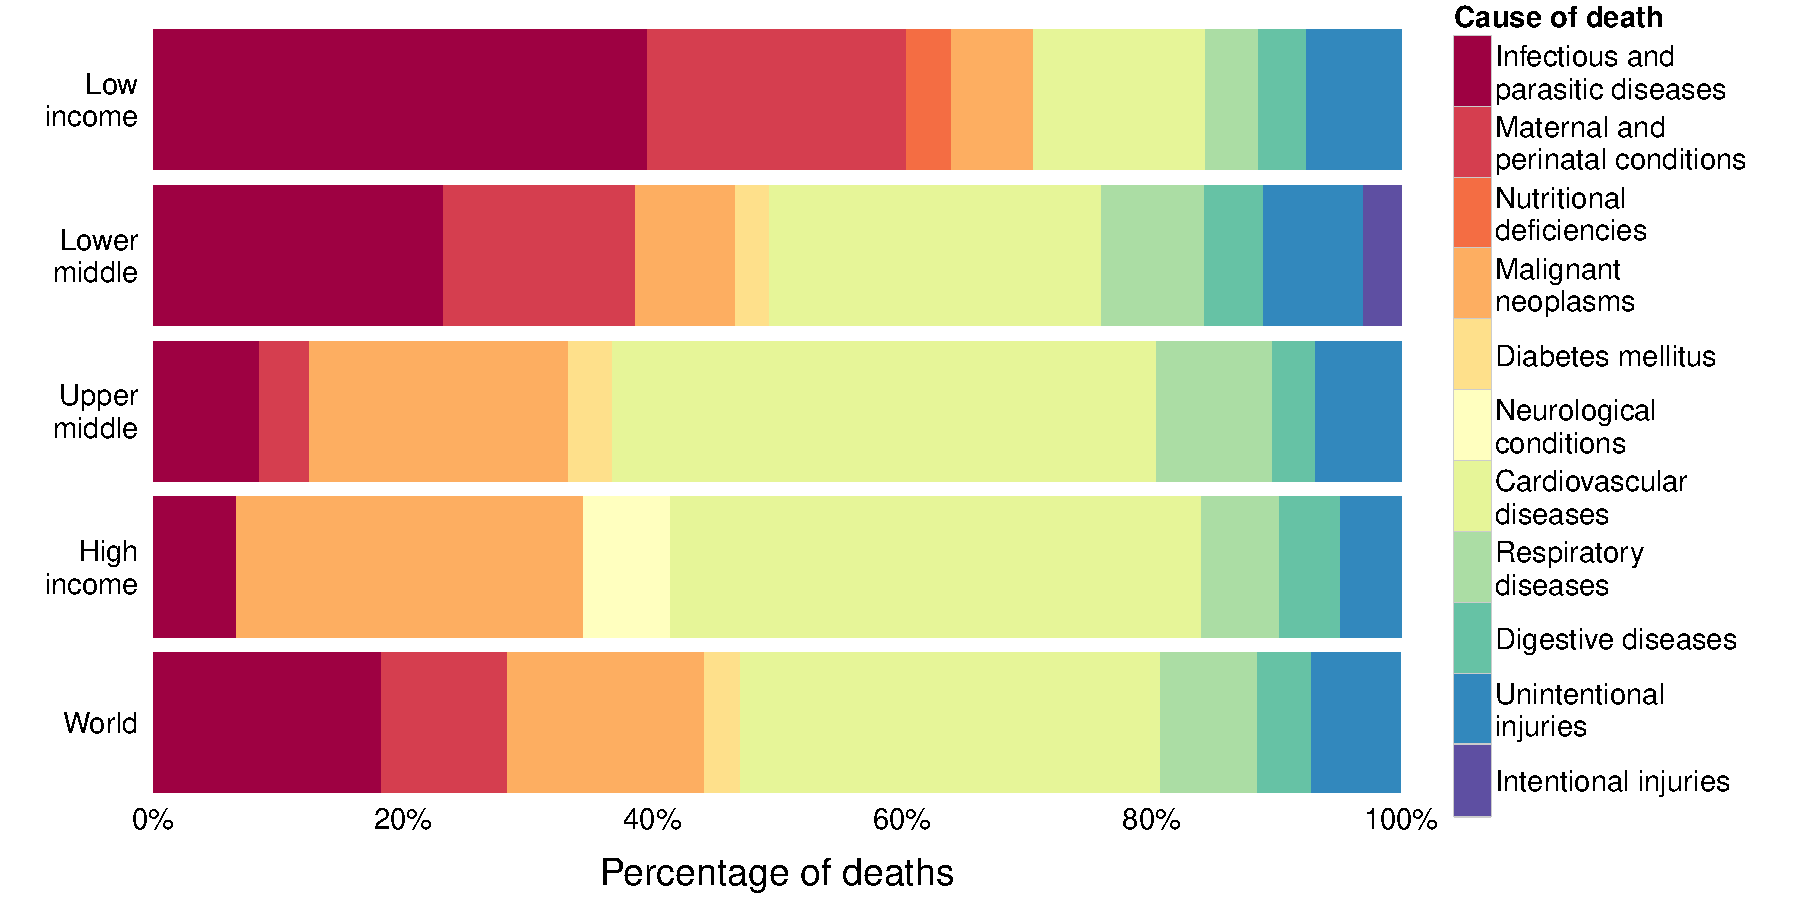
\includegraphics[width=\maxwidth]{figures/R/who-deaths/topCauses-who-deaths_top-causes-1} \caption[Relative frequencies of death causes in 2012 by World Bank income groups]{Relative frequencies of death causes in 2012 by World Bank income groups. Binning is based on Gross National Income (GNI) per capita and the thresholds are \$1'045 or less for low income, \$1046 to \$4125 for lower-middle, \$4126 to \$12745 for upper-middle and \$12746 or more for high income economies. The data was obtained from the \cite{WHO2012}.}\label{fig:who-deaths_top-causes}
\end{figure}


\end{knitrout}

\newcommand{\knitrTotalDeathsTwelve}{58.3 million}

\newcommand{\knitrPercentageDeathsTwelveHigh}{20.1\%}
\newcommand{\knitrPercentageDeathsTwelveLow}{14\%}
\newcommand{\knitrPercentageDeathsTwelveLmid}{36.5\%}
\newcommand{\knitrPercentageDeathsTwelveUmid}{29.4\%}

\newcommand{\knitrPercentDeathsTwelveLowInfect}{39.6\%}
\newcommand{\knitrPercentDeathsTwelveLowPerinat}{20.8\%}
\newcommand{\knitrPercentDeathsTwelveLmidInfect}{23.3\%}
\newcommand{\knitrPercentDeathsTwelveLmidCardio}{26.5\%}
\newcommand{\knitrPercentDeathsTwelveUmidInfect}{8.5\%}
\newcommand{\knitrPercentDeathsTwelveHighInfect}{6.7\%}
\newcommand{\knitrPercentDeathsTwelveWorldInfect}{18.3\%}
\newcommand{\knitrPercentDeathsTwelveWorldCardio}{33.7\%}


Despite development of means to treat and prevent many previously devastating diseases, infectious pathogens remain a serious threat to global health. In 2012, an estimated total of \knitrTotalDeathsTwelve{} people died (\knitrPercentageDeathsTwelveHigh{} in high, \knitrPercentageDeathsTwelveUmid{} in upper-middle, \knitrPercentageDeathsTwelveLmid{} in lower-middle and \knitrPercentageDeathsTwelveLow{} in low income countries). Figure \ref{fig:who-deaths_top-causes} partitions the total death count into World Bank income groups and causes. In low income countries, infective diseases are the most prevalent cause of death (\knitrPercentDeathsTwelveLowInfect{}), followed by maternal and perinatal complications with substantial margin (\knitrPercentDeathsTwelveLowPerinat{}). In lower middle income countries, cardiovascular conditions catch up (\knitrPercentDeathsTwelveLmidCardio{}), but are still almost matched in frequency by infectious diseases (\knitrPercentDeathsTwelveLmidInfect{}). In upper middle (\knitrPercentDeathsTwelveUmidInfect{}) and high income countries (\knitrPercentDeathsTwelveHighInfect{}), the importance of infectious disease while weakened remains accountable for a significant number of deaths. Globally, infectious diseases are the second most frequent cause of death (\knitrPercentDeathsTwelveWorldInfect{}), even more prevalent than all forms of cancer combined (\knitrPercentDeathsTwelveWorldCancer{}) and only preceded by cardiovascular diseases (\knitrPercentDeathsTwelveWorldCardio{}).

\begin{knitrout}
\definecolor{shadecolor}{rgb}{0.969, 0.969, 0.969}\color{fgcolor}\begin{figure}
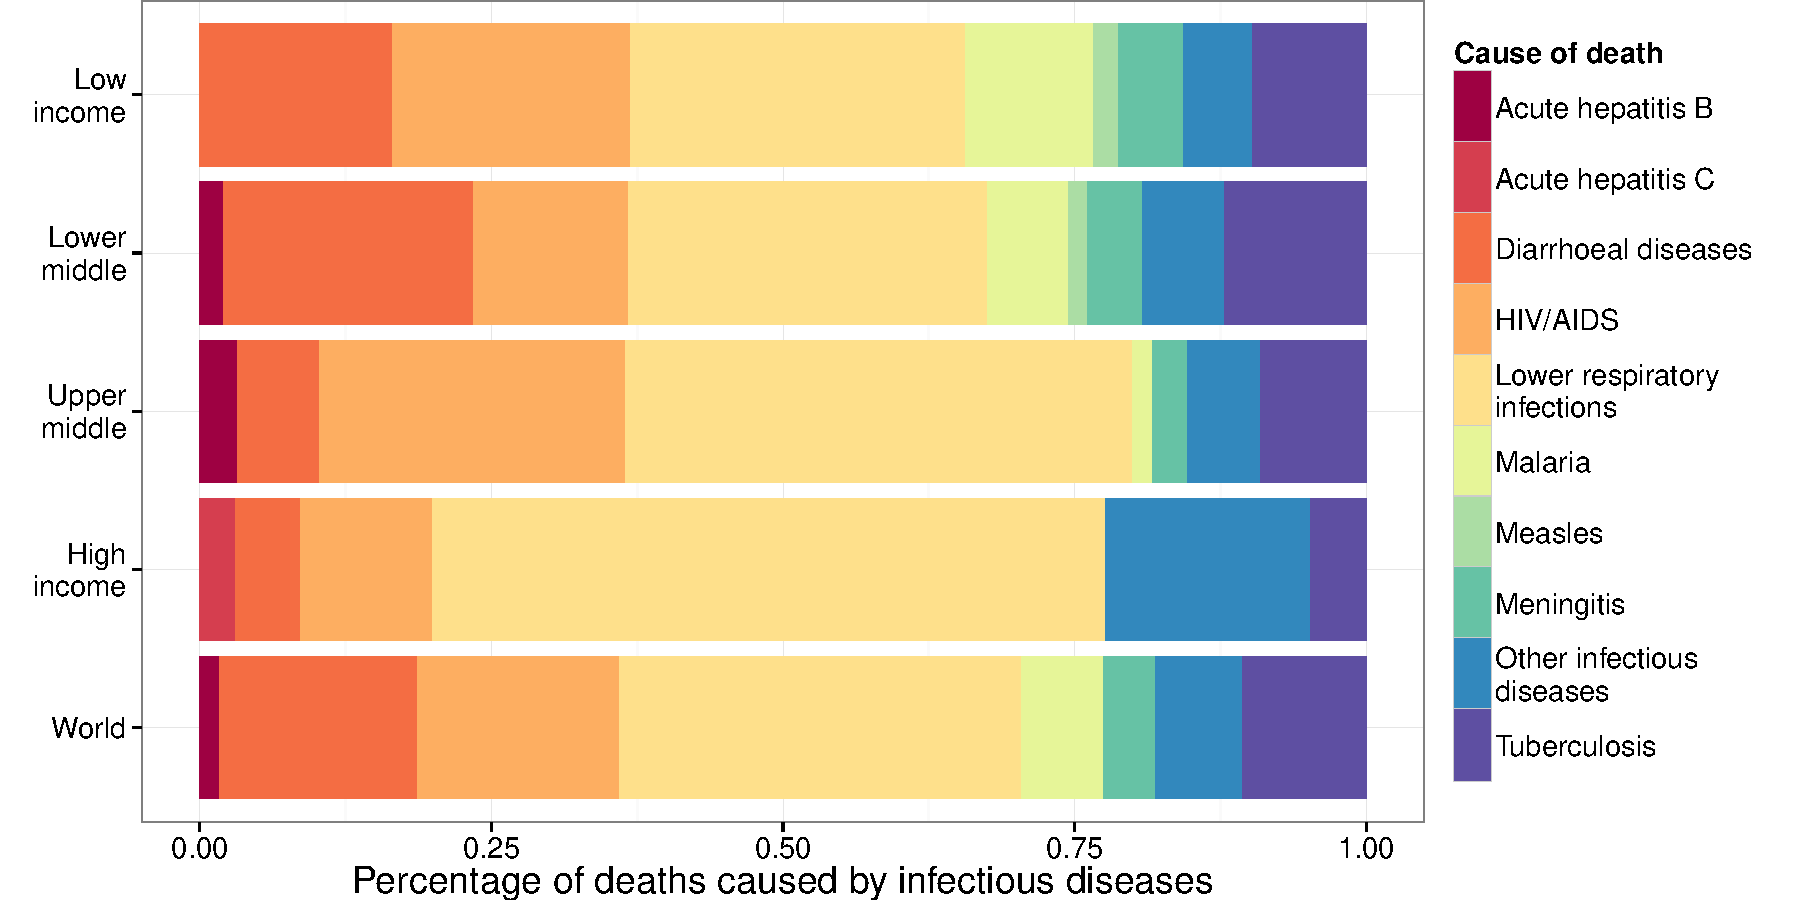
\includegraphics[width=\maxwidth]{figures/R/who-deaths/byDisease-who-deaths_by-disease-1} \caption[Relative frequencies deadly infectious diseases for 2012 by World Bank income groups]{Relative frequencies of deadly infectious diseases for 2012 by World Bank income groups. Binning is based on Gross National Income (GNI; see figure \ref{fig:who-deaths_top-causes}). The data was obtained from the \cite{WHO2012}.}\label{fig:who-deaths_by-disease}
\end{figure}


\end{knitrout}

\newcommand{\knitrPercentageInfectTwelveWorldLRI}{34.5\%}
\newcommand{\knitrPercentageInfectTwelveHighLRI}{57.7\%}
\newcommand{\knitrPercentageInfectTwelveUmidLRI}{43.5\%}
\newcommand{\knitrPercentageInfectTwelveLmidLRI}{30.8\%}
\newcommand{\knitrPercentageInfectTwelveLowLRI}{28.7\%}
\newcommand{\knitrPercentageInfectTwelveHighDiarr}{5.6\%}
\newcommand{\knitrPercentageInfectTwelveUmidDiarr}{7\%}
\newcommand{\knitrPercentageInfectTwelveLmidDiarr}{21.4\%}
\newcommand{\knitrPercentageInfectTwelveLowDiarr}{16.6\%}
\newcommand{\knitrPercentageInfectTwelveWorldAIDS}{17.3\%}
\newcommand{\knitrPercentageInfectTwelveWorldDiarr}{16.9\%}
\newcommand{\knitrPercentageInfectTwelveHighAIDS}{11.3\%}
\newcommand{\knitrPercentageInfectTwelveUmidAIDS}{26.2\%}
\newcommand{\knitrPercentageInfectTwelveLmidAIDS}{13.3\%}
\newcommand{\knitrPercentageInfectTwelveLowAIDS}{20.4\%}


Focusing only on deaths caused by infectious disease, lower respiratory infections are most frequent (for each income region individually, low to high: \knitrPercentageInfectTwelveLowLRI{}, \knitrPercentageInfectTwelveLmidLRI{}, \knitrPercentageInfectTwelveUmidLRI{} and \knitrPercentageInfectTwelveHighLRI{} as well as worldwide: \knitrPercentageInfectTwelveWorldLRI{}; cf. figure \ref{fig:who-deaths_by-disease}). Diarrhoeal diseases and \cgls{hiv}\slash \cgls{aids} are the next most common worldwide (\knitrPercentageInfectTwelveWorldDiarr{} and \knitrPercentageInfectTwelveWorldAIDS{}, respectively) where diarrhea is more prevalent in lower income regions (\knitrPercentageInfectTwelveLowDiarr{} and \knitrPercentageInfectTwelveLmidDiarr{} versus \knitrPercentageInfectTwelveUmidDiarr{} and \knitrPercentageInfectTwelveHighDiarr{}), while \cgls{hiv}\slash \cgls{aids} plays a major role irrespective of income region (low to high: \knitrPercentageInfectTwelveLowAIDS{}, \knitrPercentageInfectTwelveLmidAIDS{}, \knitrPercentageInfectTwelveUmidAIDS{} and \knitrPercentageInfectTwelveHighAIDS{}).

Dealing with highly virulent pathogens and preventing their spreading requires a multi-pronged approach. First and foremost, etiology and routes of transmission have to be understood. Knowledge of vectors and natural reservoirs is of great importance as a first line of defense. In the case of plague, for example, insecticides killing fleas were successfully used as a prophylactic measure, as was controlling rat populations \citep{Barnes1990}. Sanitary precautions including purification of drinking water, cocking foods well and the usage of disinfectants prevent initial infection, while measures such as sewage treatment, hand washing and wearing face masks help limiting spread among humans. Vaccination is the most important preventive measure. Exposing the immune system to a foreign antigen in a controlled manner artificially induces immunity. Among the great successes of widespread vaccination efforts is the global eradication of smallpox through a coordinated initiative lead by the World Health Organization in the 1970's.

Post-infection therapies include symptomatic treatments, as well as anti-in\-fec\-tive drugs. Antibiotics exploit differences in proteomes between host and pathogen to selectively disable the invader with minimal toxicity to the host. This approach has been tremendously successful throughout most of the 20th century, leading to widespread application and prompting development of resistance towards the commonly used compounds. Adding to the severity of the problem is a lack of discovery of new drugs. No new class of anti-bacterial agents has been found since 1987, causing big pharmaceutical companies to withdraw from the area. The remaining research is mainly focused on improving on existing drugs, leading to a weak product pipeline, especially for the treatment of gram-negative bacteria \citep{Silver2011}. In its first global study on anti-microbial resistance, the \citet{WHO2014} notes:

\begin{quote}
\cGls{amr} within a wide range of infectious agents is a growing public health threat of broad concern \ldots A post-antibiotic era—-in which common infections and minor injuries can kill—-far from being an apocalyptic fantasy, is instead a very real possibility for the 21st century.
\end{quote}

An alternative to pathogen directed search lies in targeting the set of host proteins necessary for infection. Many intracellular parasites subvert cellular functions to gain entry via host-mediated processes such as endocytosis. Upon entry, they move to a suitable niche and rely on host resources for proliferation. Challenges include evading host-cell defense mechanisms, generating sufficient space for replication, nutrient acquisition and keeping the host alive as long as possible, most of which require complex interactions between invader and host-based mechanisms. Finally, exiting the host cell again requires the parasite to successfully insert itself into existing signaling pathways \citep{Leiriao2004}.

\cGls{hdt} offer an escape from the conundrum of wanting to combat but not wanting to select for the surviving microbial parasites. The major challenge under this regimen is finding infectome components that are nonessential for cell survival, as orthogonality of host and infectant can no longer be exploited. Proving feasibility of the approach, \citeauthor{Czyz2014} screened a library of 640 compounds already approved by the United Stated Food and Drug Administration (USFDA or short FDA) for inducing resistance to four intracellular pathogens (\textit{Coxiella burnetii}, \textit{Legionella pneumophila}, \textit{Brucella abortus}, and \textit{Rickettsia conorii}). They found multiple drugs, not classified as antibiotics, that successfully inhibited intracellular bacterial growth while entailing only limited toxicity to THP-1 host cells. \citeauthor{Prussia2011} review the usage of genome-wide screens to study host-pathogen interactions (for \cgls{hiv} and influenza) which in turn serve as basis for rational identification of drug targets for novel host-directed antivirals. \nocite{Hawn2015}

A detailed understanding of the human infectome is of crucial importance to the development of \cgls{hdt} and may even benefit the development of new anti-microbial agents. Feasibility of systematic loss of function screens using \cgls{rna} interference methodology offers a unique opportunity to investigate complex cellular networks, making this an ideal tool for laying groundwork in combating infectious diseases. Of great importance, however, is ensuring reproducibility and comparability of such datasets, as well as ready availability to the scientific community.

Created to tackle such issues, InfectX and TargetInfectX are two successive \cgls{rtd} projects funded by SystemsX, the Swiss initiative for systems biology, contracted with identification and study of the human infectome for a set of bacterial (\textit{Bartonella henselae}, \textit{Brucella abortus}, \textit{Listeria monocytogenes}, \textit{Salmonella} typhimurium and \textit{Shigella flexneri}) and viral pathogens (adenovirus, rhinovirus and \textit{Vaccinia virus}). The central effort of generating kinome- and genome-wide \cgls{sirna} screens for each of the investigated pathogens and capturing image data followed by computational image analysis is carried out by an interdisciplinary consortium of research groups spanning the Universities of Basel and Z\"urich, the Swiss Federal institute of Technology (ETH Z\"urich), as well as the Pasteur Institute.

A wealth of data is easily generated by running computational feature recognition at single cell resolution on microscopic images which subsequently calls for sophisticated statistical analysis in order to expose biologically relevant information. This master thesis explores the single cell feature space, provides software to handle such datasets and attempts to employ \cglspl{glm} for comparing \cgls{sirna}-knockdown experiments and identifying discriminatory features. Following this introductory part, chapter 2 will provide the necessary biological background, covering microbial infection mechanisms, a description of each pathogen in terms of physical characteristics, diseases caused, pathogenesis and epidemiology, as well as giving an introduction on \cgls{rna} interference, including molecular mechanism, biological function and several applications alongside methodological caveats. Chapter 3 reviews InfectX data collection, detailing experimental setup, image acquisition, data processing and image analysis, as well as qualitatively describing the available datasets.

An R package called singleCellFeatures was developed to facilitate working with single cell feature datasets, the specifics of which are detailed in chapter 4. Beginning with a motivational example, the importance of efficient computation and data representation is highlighted and the R package is described in terms of developed S3 classes as well as data fetching, caching, manipulation and analysis routines. Finally, chapter 5 introduces \cglspl{glm}, \cglspl{pmm}, deliberates several normalization approaches and concludes with some analysis results along with a discussion of unresolved issues.


\chapter{Writing scientific texts in English}

This chapter was originally a separate document written by Reto
Spöhel.  It is reprinted here so that the template can serve as a
quick guide to thesis writing, and to provide some more example
material to give you a feeling for good typesetting.

% We're going to need an extra theorem-like environment for this
% chapter
\theoremstyle{plain}
\theoremsymbol{}
\newtheorem{Rule}[theorem]{Rule}

\section{Basic writing rules}

The following rules need little further explanation; they are best
understood by looking at the example in the booklet by Knuth et al.,
§2--§3.

\begin{Rule}
  Write texts, not chains of formulas.
\end{Rule}

More specifically, write full sentences that are logically
interconnected by phrases like `Therefore', `However', `On the other
hand', etc.\ where appropriate.

\begin{Rule}
  Displayed formulas should be embedded in your text and punctuated
  with it.
\end{Rule}

In other words, your writing should not be divided into `text parts'
and `formula parts'; instead the formulas should be tied together by
your prose such that there is a natural flow to your writing.

\section{Being nice to the reader}

Try to write your text in such a way that a reader enjoys reading
it. That's of course a lofty goal, but nevertheless one you should
aspire to!

\begin{Rule}
  Be nice to the reader.
\end{Rule}

Give some intuition or easy example for definitions and theorems which
might be hard to digest. Remind the reader of notations you introduced
many pages ago -- chances are he has forgotten them. Illustrate your
writing with diagrams and pictures where this helps the reader. Etc.

\begin{Rule}
  Organize your writing.
\end{Rule}

Think carefully about how you subdivide your thesis into chapters,
sections, and possibly subsections.  Give overviews at the beginning
of your thesis and of each chapter, so the reader knows what to
expect. In proofs, outline the main ideas before going into technical
details. Give the reader the opportunity to `catch up with you' by
summing up your findings periodically.

\emph{Useful phrases:} `So far we have shown that \ldots', `It remains
to show that \ldots', `Recall that we want to prove inequality (7), as
this will allow us to deduce that \ldots', `Thus we can conclude that
\ldots. Next, we would like to find out whether \ldots', etc.

\begin{Rule}
  Don't say the same thing twice without telling the reader that you
  are saying it twice.
\end{Rule}

Repetition of key ideas is important and helpful. However, if you
present the same idea, definition or observation twice (in the same or
different words) without telling the reader, he will be looking for
something new where there is nothing new.

\emph{Useful phrases:} `Recall that [we have seen in Chapter 5 that]
\ldots', `As argued before / in the proof of Lemma 3, \ldots', `As
mentioned in the introduction, \ldots', `In other words, \ldots', etc.

\begin{Rule}
  Don't make statements that you will justify later without telling
  the reader that you will justify them later.
\end{Rule}

This rule also applies when the justification is coming right in the
next sentence!  The reasoning should be clear: if you violate it, the
reader will lose valuable time trying to figure out on his own what
you were going to explain to him anyway.

\emph{Useful phrases:} `Next we argue that \ldots', `As we shall see,
\ldots', `We will see in the next section that \ldots, etc.


\section{A few important grammar rules}

\begin{Rule}
  \label{rule:no-comma-before-that}
  There is (almost) \emph{never} a comma before `that'.
\end{Rule}

It's really that simple. Examples:
\begin{quote}
  We assume that \ldots\\
  \emph{Wir nehmen an, dass \ldots}

  It follows that \ldots\\
  \emph{Daraus folgt, dass \ldots}

  `thrice' is a word that is seldom used.\\
  \emph{`thrice' ist ein Wort, das selten verwendet wird.}
\end{quote}
Exceptions to this rule are rare and usually pretty obvious. For
example, you may end up with a comma before `that' because `i.e.' is
spelled out as `that is':
\begin{quote}
  For \(p(n)=\log n/n\) we have \ldots{} However, if we choose \(p\) a
  little bit higher, that is \(p(n)=(1+\varepsilon)\log n/n\) for some
  \(\varepsilon>0\), we obtain that\ldots
\end{quote}
Or you may get a comma before `that' because there is some additional
information inserted in the middle of your sentence:
\begin{quote}
  Thus we found a number, namely \(n_0\), that satisfies equation (13).
\end{quote}
If the additional information is left out, the sentence has no comma:
\begin{quote}
  Thus we found a number that satisfies equation (13).
\end{quote}
(For `that' as a relative pronoun, see also
Rules~\ref{rule:non-defining-has-comma}
and~\ref{rule:defining-without-comma} below.)

\begin{Rule}
  There is usually no comma before `if'.
\end{Rule}

Example:
\begin{quote}
  A graph is not \(3\)-colorable if it contains a \(4\)-clique.\\
  \emph{Ein Graph ist nicht \(3\)-färbbar, wenn er eine \(4\)-Clique
    enthält.}
\end{quote}
However, if the `if' clause comes first, it is usually separated from
the main clause by a comma:
\begin{quote}
  If a graph contains a \(4\)-clique, it is not \(3\)-colorable .\\
  \emph{Wenn ein Graph eine \(4\)-Clique enthält, ist er nicht
    \(3\)-färbbar.}
\end{quote}

There are more exceptions to these rules than to
Rule~\ref{rule:no-comma-before-that}, which is why we are not
discussing them here. Just keep in mind: don't put a comma before `if'
without good reason.

\begin{Rule}
  \label{rule:non-defining-has-comma}
  Non-defining relative clauses have commas.
\end{Rule}
\begin{Rule}
  \label{rule:defining-without-comma}
  Defining relative clauses have no commas.
\end{Rule}

In English, it is very important to distinguish between two types of
relative clauses: defining and non-defining ones. This is a
distinction you absolutely need to understand to write scientific
texts, because mistakes in this area actually distort the meaning of
your text!

It's probably easier to explain first what a \emph{non-defining}
relative clause is. A non-defining relative clauses simply gives
additional information \emph{that could also be left out} (or given in
a separate sentence). For example, the sentence
\begin{quote}
  The \textsc{WeirdSort} algorithm, which was found by the famous
  mathematician John Doe, is theoretically best possible but difficult
  to implement in practice.
\end{quote}
would be fully understandable if the relative clause were left out
completely. It could also be rephrased as two separate sentences:
\begin{quote}
  The \textsc{WeirdSort} algorithm is theoretically best possible but
  difficult to implement in practice. [By the way,] \textsc{WeirdSort}
  was found by the famous mathematician John Doe.
\end{quote}
This is what a non-defining relative clause is. \emph{Non-defining
  relative clauses are always written with commas.} As a corollary we
obtain that you cannot use `that' in non-defining relative clauses
(see Rule~\ref{rule:no-comma-before-that}!). It would be wrong to
write
\begin{quote}
  \st{The \textsc{WeirdSort} algorithm, that was found by the famous
    mathematician John Doe, is theoretically best possible but
    difficult to implement in practice.}
\end{quote}
A special case that warrants its own example is when `which' is
referring to the entire preceding sentence:
\begin{quote}
  Thus inequality (7) is true, which implies that the Riemann
  hypothesis holds.
\end{quote}
As before, this is a non-defining relative sentence (it could be left
out) and therefore needs a comma.

So let's discuss \emph{defining} relative clauses next. A defining
relative clause tells the reader \emph{which specific item the main
  clause is talking about}. Leaving it out either changes the meaning
of the sentence or renders it incomprehensible altogether.  Consider
the following example:

\begin{quote}
  The \textsc{WeirdSort} algorithm is difficult to implement in
  practice. In contrast, the algorithm that we suggest is very simple.
\end{quote}

Here the relative clause `that we suggest' cannot be left out -- the
remaining sentence would make no sense since the reader would not know
which algorithm it is talking about. This is what a defining relative
clause is. \textit{Defining relative clauses are never written with
  commas.} Usually, you can use both `that' and `which' in defining
relative clauses, although in many cases `that' sounds better.

As a final example, consider the following sentence:
\begin{quote}
  For the elements in \(\mathcal{B}\) which satisfy property (A), we
  know that equation (37) holds.
\end{quote}
This sentence does not make a statement about all elements in
\(\mathcal{B}\), only about those satisfying property (A). The relative
clause is \emph{defining}. (Thus we could also use `that' in place of
`which'.)

In contrast, if we add a comma the sentence reads
\begin{quote}
  For the elements in \(\mathcal{B}\), which satisfy property (A), we
  know that equation (37) holds.
\end{quote}

Now the relative clause is \emph{non-defining} -- it just mentions in
passing that all elements in \(\mathcal{B}\) satisfy property (A). The
main clause states that equation (37) holds for \emph{all} elements in
\(\mathcal{B}\). See the difference?


\section[Things you (usually) don't say in English]%
{Things you (usually) don't say in English -- and what to say
  instead}
\label{sec:list}

Table~\ref{tab:things-you-dont-say} lists some common mistakes and
alternatives.  The entries should not be taken as gospel -- they don't
necessarily mean that a given word or formulation is wrong under all
circumstances (obviously, this depends a lot on the context). However,
in nine out of ten instances the suggested alternative is the better
word to use.

\begin{table}
  \centering
  \caption{Things you (usually) don't say}
  \label{tab:things-you-dont-say}
  \begin{tabular}{lll}
    \toprule
    \st{It holds (that) \dots} & We have \dots & \emph{Es gilt \dots}\\
    \multicolumn{3}{l}{\quad\footnotesize(`Equation (5) holds.' is fine, though.)}\\
    \st{$x$ fulfills property $\mathcal{P}$.}& \(x\) satisfies property \(\mathcal{P}\). & \emph{\(x\) erfüllt Eigenschaft \(\mathcal{P}\).} \\
    \st{in average} & on average & \emph{im Durchschnitt}\\
    \st{estimation} & estimate   & \emph{Abschätzung}\\
    \st{composed number} & composite number & \emph{zusammengesetzte Zahl}\\
    \st{with the help of} & using & \emph{mit Hilfe von}\\
    \st{surely} & clearly & \emph{sicher, bestimmt}\\
    \st{monotonously increasing} & monotonically incr. & \emph{monoton steigend}\\
    \multicolumn{3}{l}{\quad\footnotesize(Actually, in most cases `increasing' is just fine.)}\\
    \bottomrule
  \end{tabular}
\end{table}

%%% Local Variables:
%%% mode: latex
%%% TeX-master: "thesis"
%%% End:

\chapter{Typography}


\section{Punctuation}

\begin{Rule}
  Use opening (`) and closing (') quotation marks correctly.
\end{Rule}

In \LaTeX, the closing quotation mark is typed like a normal
apostrophe, while the opening quotation mark is typed using the French
\emph{accent grave} on your keyboard (the \emph{accent grave} is the
one going down, as in \emph{frère}).

Note that any punctuation that \emph{semantically} follows quoted
speech goes inside the quotes in American English, but outside in
Britain.  Also, Americans use double quotes first.  Oppose
\begin{quote}
  ``Using `lasers,' we punch a hole in \ldots\ the Ozone Layer,''
  Dr.\ Evil said.
\end{quote}
to
\begin{quote}
  `Using ``lasers'', we punch a hole in \ldots\ the Ozone Layer',
  Dr.\ Evil said.
\end{quote}

\begin{Rule}
  Use hyphens (-), en-dashes (--) and em-dashes (---) correctly.
\end{Rule}

A hyphen is only used in words like `well-known', `$3$-colorable'
etc., or to separate words that continue in the next line (which is
known as hyphenation).  It is entered as a single ASCII hyphen
character (\texttt{-}).

To denote ranges of numbers, chapters, etc., use an en-dash (entered
as two ASCII hyphens \texttt{--}) with no spaces on either side.  For
example, using Equations (1)--(3), we see\ldots

As the equivalent of the German \emph{Gedankenstrich}, use an en-dash
with spaces on both sides -- in the title of Section \ref{sec:list},
it would be wrong to use a hyphen instead of the dash. (Some English
authors use the even longer emdash (---) instead, which is typed as
three subsequent hyphens in \LaTeX. This emdash is used without spaces
around it---like so.)


\section{Spacing}

\begin{Rule}
  \label{rule:no-manual-spacing}
  Do not add spacing manually.
\end{Rule}

You should never use the commands \lstinline-\\- (except within
tabulars and arrays), \lstinline[showspaces=true]-\ - (except to
prevent a sentence-ending space after Dr.\ and such),
\lstinline-\vspace-, \lstinline-\hspace-, etc.  The choices programmed
into \LaTeX{} and this style should cover almost all cases.  Doing it
manually quickly leads to inconsistent spacing, which looks terrible.
Note that this list of commands is by no means conclusive.

\begin{Rule}
  Judiciously insert spacing in maths where it helps.
\end{Rule}

This directly contradicts Rule~\ref{rule:no-manual-spacing}, but in
some cases \TeX{} fails to correctly decide how much spacing is
required.  For example, consider
\begin{displaymath}
  f(a,b) = f(a+b, a-b).
\end{displaymath}
In such cases, inserting a thin math space \lstinline-\,- greatly
increases readability:
\begin{displaymath}
  f(a,b) = f(a+b,\, a-b).
\end{displaymath}

Along similar lines, there are variations of some symbols with
different spacing.  For example, Lagrange's Theorem states that
\(\abs{G}=[G:H]\abs{H}\), but the proof uses a bijection \(f\colon
aH\to bH\).  (Note how the first colon is symmetrically spaced, but
the second is not.)

\begin{Rule}
  Learn when to use \lstinline[showspaces=true]-\ - and
  \lstinline-\@-.
\end{Rule}

Unless you use `french spacing', the space at the end of a sentence is
slightly larger than the normal interword space.

The rule used by \TeX{} is that any space following a period,
exclamation mark or question mark is sentence-ending, except for
periods preceded by an upper-case letter.  Inserting \lstinline-\-
before a space turns it into an interword space, and inserting
\lstinline-\@- before a period makes it sentence-ending.  This means
you should write
\begin{lstlisting}
Prof.\ Dr.\ A. Steger is a member of CADMO\@.
If you want to write a thesis with her, you
should use this template.
\end{lstlisting}
which turns into
\begin{quote}
  Prof.\ Dr.\ A. Steger is a member of CADMO\@.  If you want to write
  a thesis with her, you should use this template.
\end{quote}
The effect becomes more dramatic in lines that are stretched slightly
during justification:
\begin{quote}
  \parbox{\linewidth}{\hbox to \linewidth{%
      Prof.\ Dr.\ A. Steger is a member of CADMO\@.  If you}}
\end{quote}

\begin{Rule}
  Place a non-breaking space (\lstinline-~-) right before references.
\end{Rule}

This is actually a slight simplification of the real rule, which
should invoke common sense.  Place non-breaking spaces where a line
break would look `funny' because it occurs right in the middle of a
construction, especially between a reference type (Chapter) and its
number.


\section{Choice of `fonts'}

Professional typography distinguishes many font attributes, such as
family, size, shape, and weight.  The choice for sectional divisions
and layout elements has been made, but you will still occasionally
want to switch to something else to get the reader's attention.  The
most important rule is very simple.

\begin{Rule}
  When emphasising a short bit of text, use \lstinline-\emph-.
\end{Rule}

In particular, \emph{never} use bold text (\lstinline-\textbf-).
Italics (or Roman type if used within italics) avoids distracting the
eye with the huge blobs of ink in the middle of the text that bold
text so quickly introduces.

Occasionally you will need more notation, for example, a consistent
typeface used to identify algorithms.

\begin{Rule}
  Vary one attribute at a time.
\end{Rule}

For example, for \textsc{WeirdSort} we only changed the shape to small
caps.  Changing two attributes, say, to bold small caps would be
excessive (\LaTeX{} does not even have this particular variation).
The same holds for mathematical notation: the reader can easily
distinguish \(g_n\), \(G(x)\), \(\mathcal{G}\) and \(\mathsf{G}\).

\begin{Rule}
  Never underline or uppercase.
\end{Rule}

No exceptions to this one, unless you are writing your thesis on a
typewriter.  Manually.  Uphill both ways.  In a blizzard.


\section{Displayed equations}

\begin{Rule}
  Insert paragraph breaks \emph{after} displays only where they
  belong.  Never insert paragraph breaks \emph{before} displays.
\end{Rule}

\LaTeX{} translates sequences of more than one linebreak (i.e., what
looks like an empty line in the source code) into a paragraph break in
almost all contexts.  This also happens before and after displays,
where extra spacing is inserted to give a visual indication of the
structure.  Adding a blank line in these places may look nice in the
sources, but compare the resulting display

\begin{displaymath}
  a = b
\end{displaymath}

to the following:
\begin{displaymath}
  a = b
\end{displaymath}
The first display is surrounded by blank lines, but the second is not.
It is bad style to start a paragraph with a display (you should always
tell the reader what the display means first), so the rule follows.

\begin{Rule}
  Never use \lstinline-eqnarray-.
\end{Rule}

It is at the root of most ill-spaced multiline displays.  The
\package{amsmath} package provides better alternatives, such as the
\lstinline-align- family
\begin{align*}
  f(x) &= \sin x, \\
  g(x) &= \cos x,
\end{align*}
and \lstinline-multline- which copes with excessively long equations:
\begin{multline*}
  \def\P{\mathrm P}
  \P\bigl[X_{t_0} \in (z_0, z_0+dz_0],\ldots, X_{t_n}\in(z_n,z_n+dz_n]\bigr]
  \\= \nu(dz_0) K_{t_1}(z_0,dz_1) K_{t_2-t_1}(z_1,dz_2)\cdots
  K_{t_n-t_{n-1}}(z_{n-1},dz_n).
\end{multline*}


\section{Floats}

By default this style provides floating environments for tables and
figures.  The general structure should be as follows:
\begin{lstlisting}
\begin{figure}
  \centering
  % content goes here
  \caption{A short caption}
  \label{some-short-label}
\end{figure}
\end{lstlisting}
Note that the label must follow the caption, otherwise the label will
refer to the surrounding section instead.  Also note that figures
should be captioned at the bottom, and tables at the top.

The whole point of floats is that they, well, \emph{float} to a place
where they fit without interrupting the text body.  This is a frequent
source of confusion and changes; please leave it as is.

\begin{Rule}
  Do not restrict float movement to only `here'
  \textnormal{(\lstinline-h-)}.
\end{Rule}

If you are still tempted, you should avoid the float altogether and
just show the figure or table inline, similar to a displayed equation.

%%% Local Variables:
%%% mode: latex
%%% TeX-master: "thesis"
%%% End:

\chapter{Example Chapter}

Dummy text.

\section{Example Section}

Dummy text.

\subsection{Example Subsection}

Dummy text.

\subsubsection{Example Subsubsection}

Dummy text.

\paragraph{Example Paragraph}

Dummy text.

\subparagraph{Example Subparagraph}

Dummy text.


\appendix

\chapter{Dummy Appendix}

You can defer lengthy calculations that would otherwise only interrupt
the flow of your thesis to an appendix.


\backmatter

\bibliographystyle{plain}
\bibliography{refs}

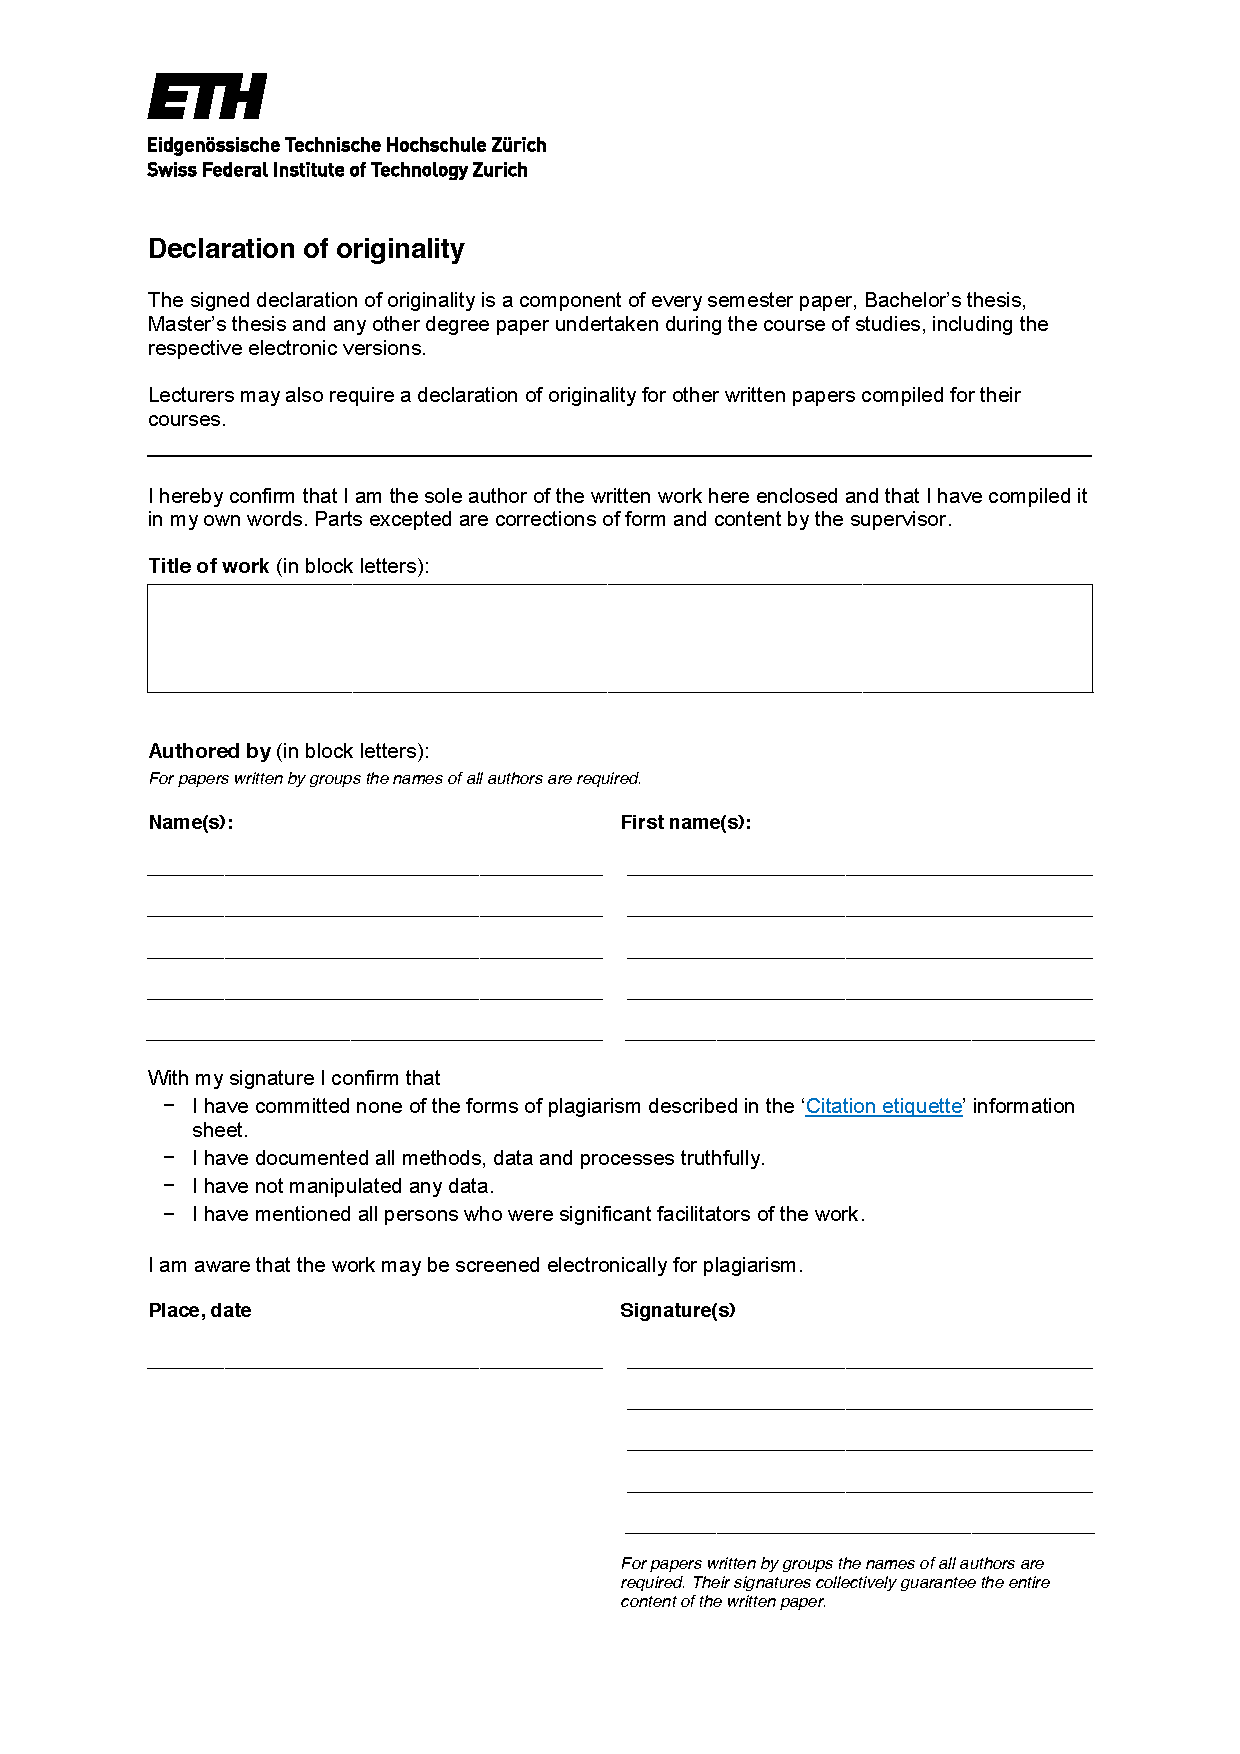
\includepdf[pages={-}]{declaration-originality.pdf}

\end{document}
